\documentclass[a4paper,12pt,twoside]{article}
\usepackage[a4paper,top=25mm,bottom=25mm,left=35mm,right=25mm]{geometry}
\usepackage[utf8]{inputenc}
\usepackage{graphicx}
\usepackage{ifpdf}
\usepackage[table]{xcolor}
%\usepackage{floatflt, rotating, latexsym, amssymb, pstcol}
\usepackage{amsmath,amsthm}
\usepackage{listings}
\usepackage{graphicx}
\usepackage{epsfig, rotating, latexsym, amssymb, pstricks}
\usepackage[numbers]{natbib}
\usepackage{setspace} 
%\usepackage[tight,footnotesize]{subfigure}
\usepackage{array}
\usepackage{overpic}
% define column for aligning numbers in tables
\usepackage{dcolumn}
\newcolumntype{d}[1]{D{.}{.}{#1}}
\usepackage{wrapfig}

\usepackage[caption=false,font=footnotesize]{subfig}
% \usepackage{natbib}
\usepackage[slovene,english]{babel}
%\usepackage[bookmarks, colorlinks=true, plainpages=false, 
%            citecolor=blue, linkcolor=blue, filecolor=blue]{hyperref}
\usepackage[bookmarks, colorlinks=true, plainpages=false,
            citecolor=black, linkcolor=black, filecolor=black,
            breaklinks=true]{hyperref}
\usepackage{bashful}
% do not reset footnote numbers for each chapter
\usepackage{chngcntr}

\usepackage[none]{hyphenat} %to prevent word splitting

\setlength\bibsep{6pt}
\setlength{\parindent}{0em}

\newenvironment{scriptdata}%
  {\vspace{3mm}\begin{list}{$\bullet$}{%
        \renewcommand{\makelabel}[1]{\textbf{##1}\hfil}%
        \setlength{\labelwidth}{17mm}%
        \setlength{\labelsep}{1mm}%
        \setlength{\leftmargin}{18mm}%
        \setlength{\itemsep}{0mm}%
        \setlength{\topsep}{0mm}%
        \setlength{\partopsep}{0mm}%
        \setlength{\parskip}{0mm}%
        \setlength{\parsep}{0mm}}}
  {\end{list}\vspace{3mm}}
  


\begin{document}

\pagestyle{plain}
\addtolength{\baselineskip}{0.4ex} % Dodatni razmik med vrsticami

% Define pagestyle
\renewcommand{\sectionmark}[1]{\markright{\thesection\ \ #1}}

% from now on, add extra line between paragraphs
\addtolength{\parskip}{\baselineskip}
%\doublespacing


\title{Edge cpo2ids converter\\work notes}
\author{Dejan Penko}
\date{\today}%April 2016}

\thispagestyle{empty}
\makeatletter
\begin{titlepage}     % Naslovna stran
  \begin{center} \bfseries
    {\large UNIVERSITY OF LJUBLJANA \par}
    \vskip 1em
    {\large Faculty of Mechanical Engineering\par}
%    \includegraphics[width=0.4\textwidth]{uni-lj-fs-logo}
    \vfill\vfill\vfill
    {\Large \textsf{\@title } \par}
    \vskip 1.5em
    %{\large \textsf{Master Thesis}}
    %\vskip 1.5em
%    Predlo\v{z}il Fakulteti za strojni\v{s}tvo Univerze v Ljubljani za dosego\\
%    akademske stopnje doktorja znanosti s podro\v{c}ja strojni\v{s}tva
    %ubmitted to the Faculty of Mechanical Engineering \\
    %of the University of Ljubljana\\
    %for the acquirement of a scientific degree of Master of Science
	%vfill
    {\Large \textsf{\@author}}
    \vfill
    %Mentor: Doc.~dr.~Leon Kos
    %\\[5mm]
    %Co-mentor: Prof.~dr.~Jo\v{z}ef Duhovnik \\[10mm]
    \vfill
    Ljubljana, \@date
  \end{center}
\end{titlepage}
\makeatother
\newpage
\graphicspath{ {images/} }

\singlespacing
\tableofcontents
\clearpage
\listoffigures
\clearpage

\section{\textbf{Introduction}}
\label{sec:introduction}


Our goal was to create a converter which will serve us for data transfer between the \emph{Edge} CPO and the \emph{Edge\_profiles} IDS database. Test data transfer was done on g04.efda-itm using two different CPO databases, the first being Shot: 16151; Run: 1000; User: kosl; Tokamak: aug; converting to IDS database Shot: 16151; Run: 1000, and the second CPO database Shot: 1; Run: 1; User: kosl; Tokamak: iter; converting to IDS database Shot: 1; Run: 1.

This document is split in two main chapters. In the first chapter we'll talk about using converter (needed modules, run command etc.) and in the second chapter about the CPO and IDS data structure and converting process, where first we will cover subgrids base information, then geometry regarding the subgrids and lastly values (as in electron density, electron temperature, ion density and ion temperature) regarding the subgrids. In each section we'll talk about data structure and converting the data from CPO to IDS database.

To avoid any confusion with index counting (python, C++ index counting starts with 0, while in Fortran starts with 1) we'll be using Fortran counting for the purposes of this working paper, which is also used in CPO database description.


\clearpage
\section{How to use cpo2ids converter}

In order for the converter to work the following modules must be loaded (using terminal):

\begin{itemize}
\item[] \%module use -a ~dkaljun/imas/etc/modulefiles
\item[] \%module load imas/develop/3/ual/develop\\ \\
Additional commands to check available modules etc.:
\item[] \%module avail imas
\item[] \%module display imas/develop/3/ual/develop
\end{itemize}

Then to run the converter \footnote[1]{found in $/pfs/work/kosl/solps-iter-ids/modules/B2.5/src/ids$)} use the command

\begin{itemize}
\item[] \%python cpo2ids.py $--$shot=16151 $--$run=1000 $--$user=kosl $--$tokamak=aug $--$version=4.10a
\end{itemize}

The $shot$, $run$, $user$, $tokamak$ and $verison$ variable has to be correctly defined in order to get access to desired database. The order of the variables can be random, only the $\%python cpo2ids.py$ has to be in the start of the command.
For now for writing to IDS the $shot$ and $run$ parameters are the same as of the CPO's. If needed that can be changed in the future.

When the converter is done the resulting files are stored in $\$HOME/public/imasdb/solps-iter/3/0$
as $ids_161511000$ (ids\_shotNumber\_runNumber).

\clearpage

\section{CPO and IDS data structure and converting process explained in depth}

\subsection{\textbf{Subgrids}}

\subsubsection{What is a subgrid?}

Briefly, grid consists of subgrids\footnote[1]{In CPO its used term $subgrid$, while in IDS it's used term $subset$} which represents all data regarding the Tokamak: geometry and values. The subgrids are the pieces that give us the whole form and/or split bigger subgrids into smaller ones. For example, subgrid $Cells$ is a whole of subgrids $Core$, $SOL$, $Inner$  $divertor$ and $Outer$ $divertor$. So if we are interested only in tokamak core data, we can choose $Core$ subgrid instead of the $Cells$ subgrid, as seen in Fig. \ref{fig:ids_Cells_te} and \ref{fig:ids_Core_te}.
Subgrids are of different classes. Class 1 is for $nodes$, class 2 for $edges$ and class 3 for 2D $cells/faces$.

\begin{figure}[!htb] \centering
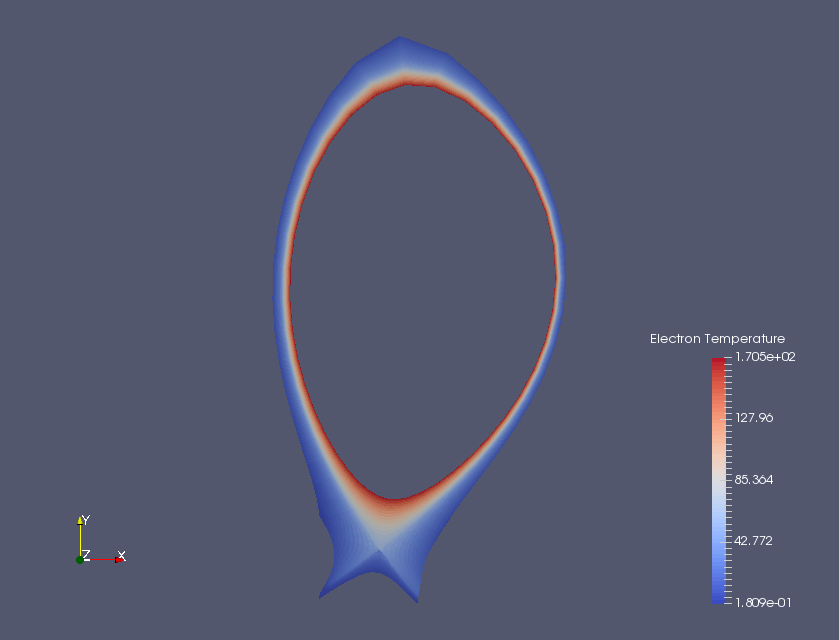
\includegraphics[scale=0.4,trim=0cm 0cm 0cm 0cm,clip]{IDS_ReadUALEdge_Cells_Subgrid}
	\caption{Cells subgrid showing electron temperature values (using IDS database)}
	\label{fig:ids_Cells_te}
\end{figure}

\clearpage
\begin{figure}[t] \centering
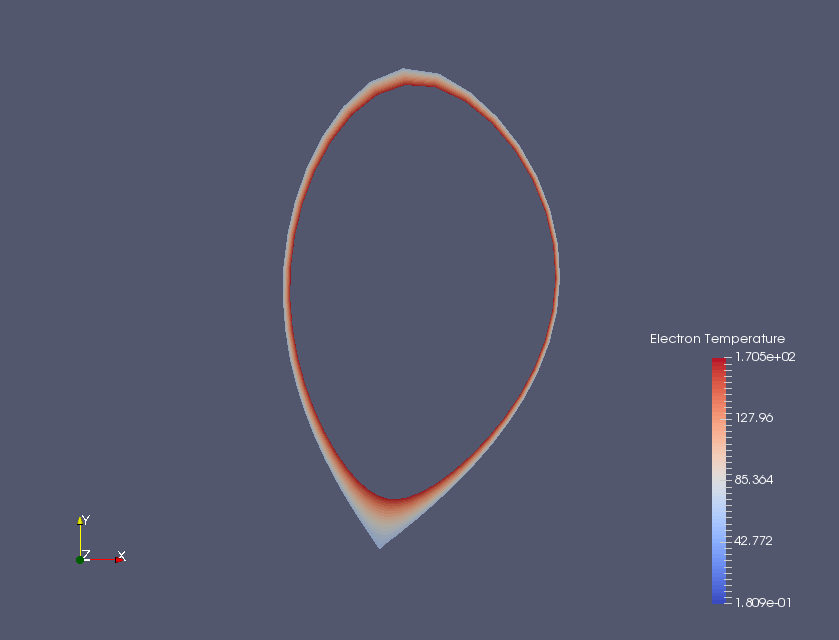
\includegraphics[scale=0.4,trim=0cm 0cm 0cm 0cm,clip]{IDS_ReadUALEdge_Core_Subgrid}
	\caption{Core subgrid showing electron temperature values (using IDS database)}
	\label{fig:ids_Core_te}
\end{figure}
\
\clearpage
\subsubsection{Subgrids structure in CPO database}
In CPO database, subgrid base parameters and indices regarding nodes, edges and cells are stored in $edge.grid.subgrid(i)$, as seen in Fig. \ref{fig:cpo_grid}, where $i$ is \textbf{subgrid base index} going from $1...n$, $n$ is sum of all subgrids. 

The $.subgrids$ subdata holds subgrid name in $.id$ and  \textbf{list of indices}, as seen in Fig. \ref{fig:cpo_subgrids}, either in \textbf{range} form found in $.list(1).indset(1).range$ or \textbf{list} form found in $.list(1).ind(j)$ together with \textbf{subgrid class} located in $.list(1).cls$ (1 for nodes, 2 for edges and 3 for cells) as seen in Fig. \ref{fig:cpo_list}, where $j$ is  number of all indices for given subgrid. 

The found indices correspond to the "main" subgrid of the same class. For example, $Core$ of subgrid class 3 corresponds to the main subgrid of the same class $Cells$. Other "main" subgrids are $Nodes$ for class 1 subgrids and $Edges$ for class 2 subgrids.

\begin{figure}[ht] \centering
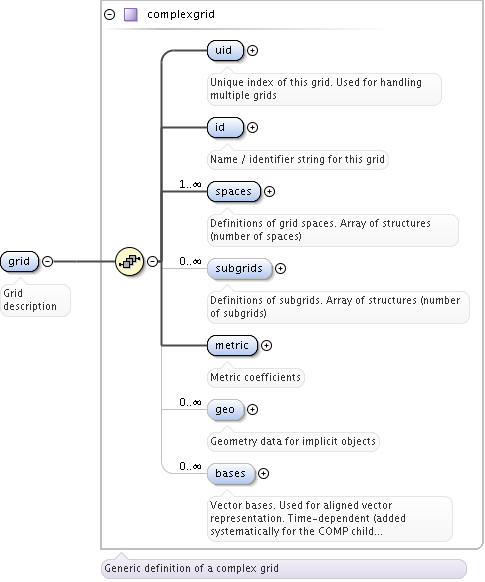
\includegraphics[scale=0.69,trim=0cm 0cm 0cm 0cm,clip]{edge_xsd_Element_grid}
	\caption{CPO $grid$ structure}
	\label{fig:cpo_grid}
\end{figure}

\begin{figure}[!htb] \centering
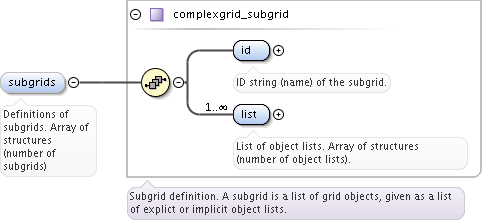
\includegraphics[scale=0.7,trim=0cm 0cm 0cm 0cm,clip]{utilities_xsd_Element_subgrids}
	\caption{CPO $subgrids$ structure}
	\label{fig:cpo_subgrids}
\end{figure}
\
\begin{figure}[!htb] \centering
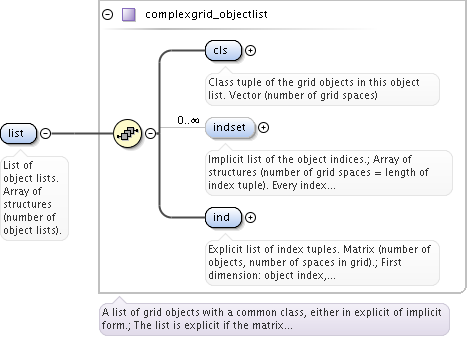
\includegraphics[scale=0.7,trim=0cm 0cm 0cm 0cm,clip]{utilities_xsd_Element_list}
	\caption{CPO $list$ structure}
	\label{fig:cpo_list}
\end{figure}
\
\clearpage

\subsubsection{Subgrids structure in IDS database}
IDS subgrid base parameters, used to determine geometry data of subgrids, are stored in location $edge\_profiles.ggd(1).grid.grid\_subset(i)$, where $i$ is \textbf{subgrid base index} going from, the same as in CPO, $1...n$, where $n$ is sum of all subgrids, as seen in Fig. \ref{fig:ids_grid}.

\begin{figure}[ht] \centering
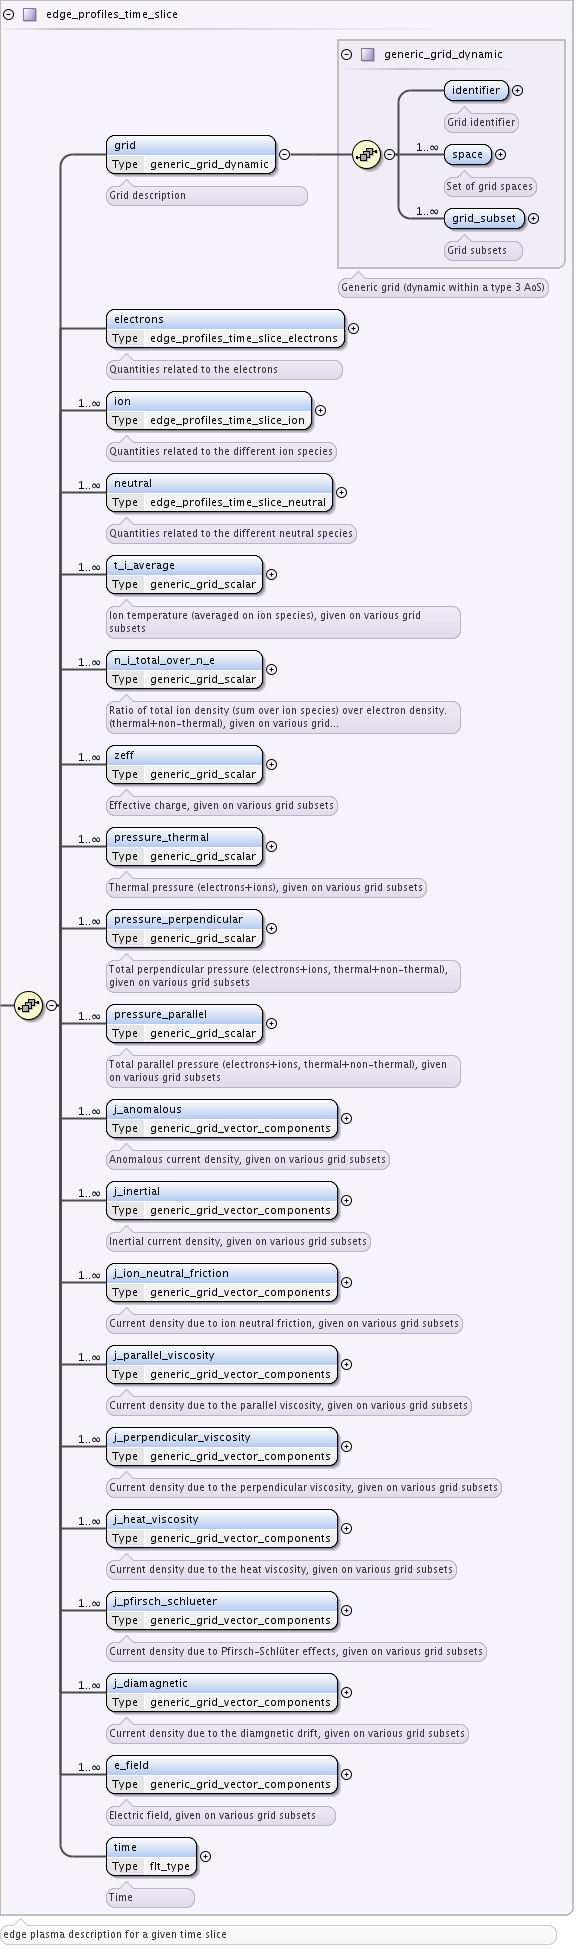
\includegraphics[scale=0.7,trim=2.5cm 58cm 0cm 1.1cm,clip]{dd_edge_profiles_edge_profiles_time_slice0}
	\caption{IDS $grid$ structure}
	\label{fig:ids_grid}
\end{figure}


It holds \textbf{subgrid name} in $.identifier.name$ and additional info \textbf{subgrid base index} in $.identifier.index$, as seen in Fig.\ref{fig:ids_subset} and \ref{fig:ids_identifier}. 
\clearpage
\begin{figure}[!htb] \centering
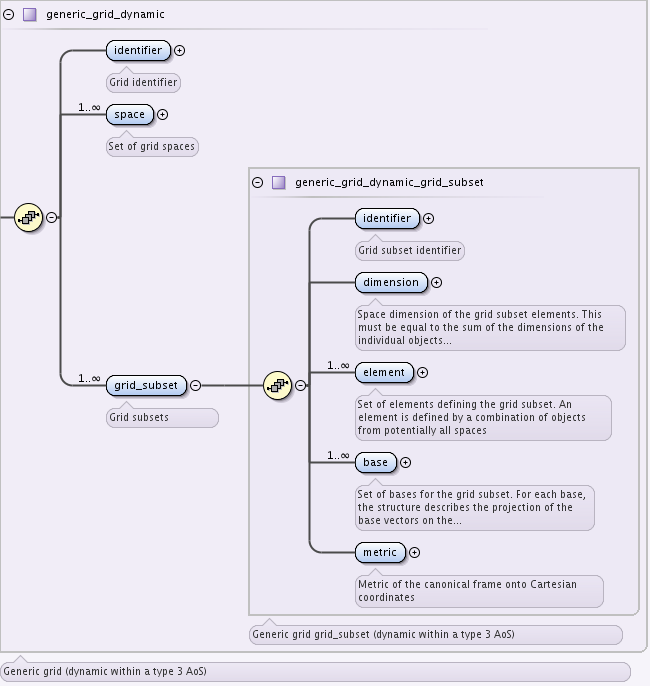
\includegraphics[scale=0.60,trim=2.5cm 1.25cm 0cm 5.7cm,clip]{dd_edge_profiles_generic_grid_dynamic_grid_subset}
	\caption{IDS $subset$ structure}
	\label{fig:ids_subset}
\end{figure}
\
\begin{figure}[!htb] \centering
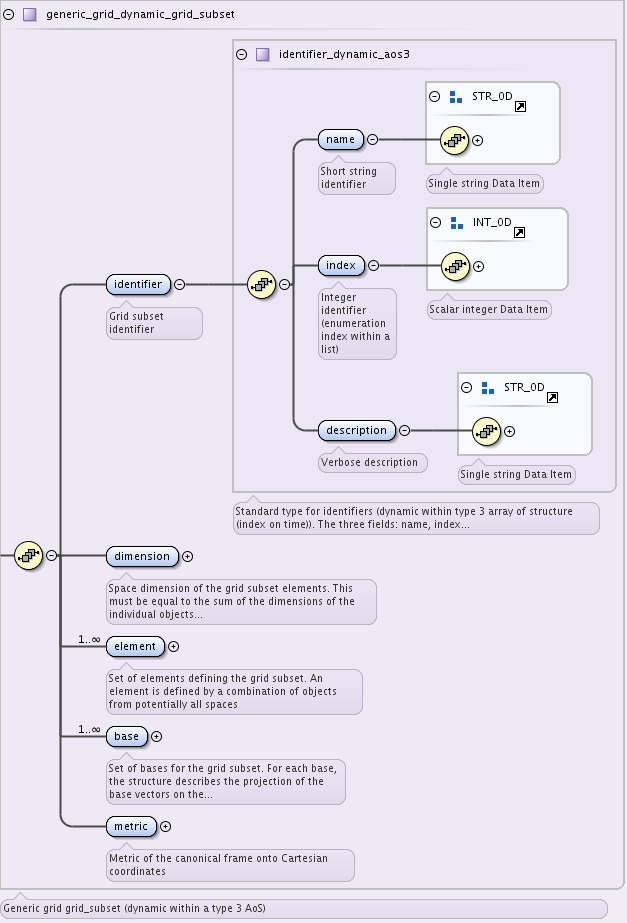
\includegraphics[scale=0.60, trim=2.8cm 13.5cm 0cm 1.1cm,clip]{dd_edge_profiles_generic_grid_dynamic_grid_subset2}
	\caption{IDS $identifier$ structure}
	\label{fig:ids_identifier}
\end{figure}
\
\clearpage
Furthermore, as seen in Fig. \ref{fig:ids_element} and \ref{fig:ids_dimension} in $.element(1).object(1).dimension$ it holds \textbf{subgrid class} and in $.element(1).object(1).index$ it holds \textbf{subgrid object index}, used to navigate to subgrids geometry data, which will be covered later.

\begin{figure}[ht] \centering
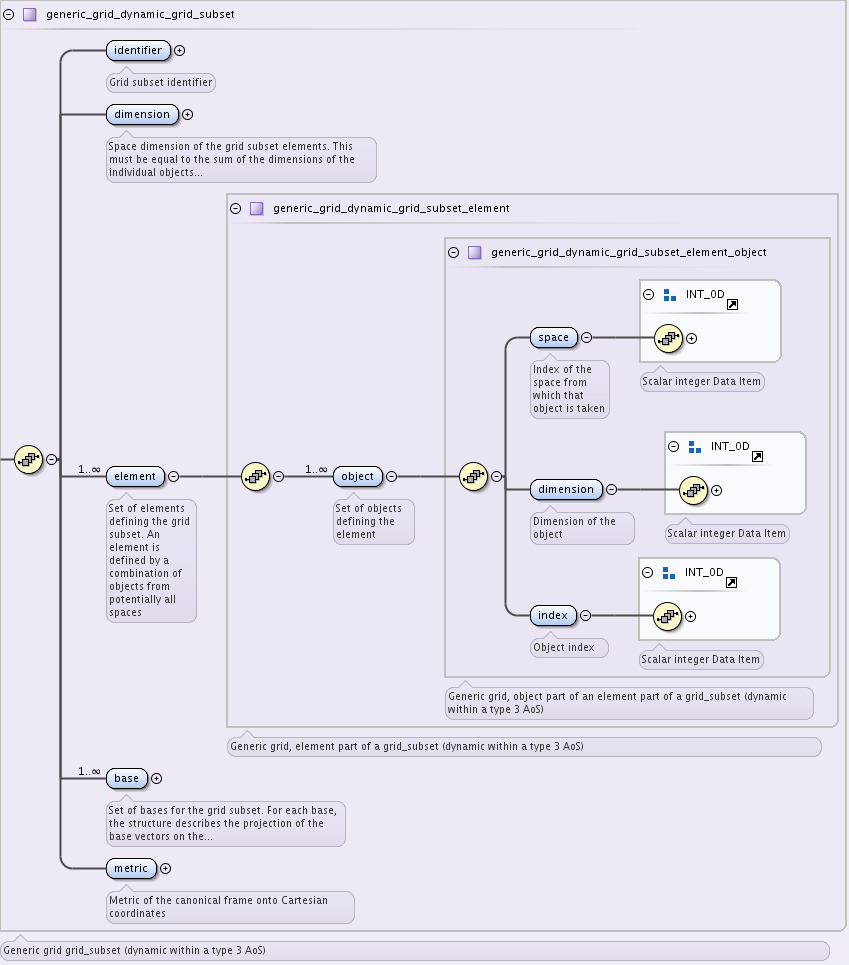
\includegraphics[scale=0.55,trim=2.5cm 7.2cm 0cm 6.5cm,clip]{dd_edge_profiles_generic_grid_dynamic_grid_subset_element}
	\caption{IDS $element$ structure}
	\label{fig:ids_element}
\end{figure}

\begin{figure}[ht] \centering
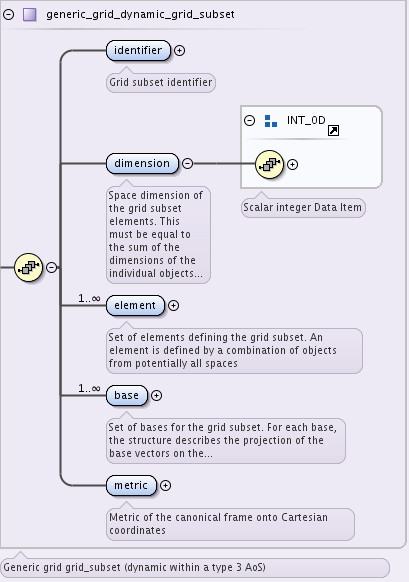
\includegraphics[scale=0.7,trim=3cm 10.4cm 0cm 3.5cm,clip]{dd_edge_profiles_generic_grid_dynamic_grid_subset3}
	\caption{IDS $dimension$ structure}
	\label{fig:ids_dimension}
\end{figure}

\clearpage 
In IDS we have one new important parameter found in $.element(1).object(1).index$. It holds \textbf{subgrid class object index}, which is $1...n$, where $n$ is sum of all subgrids of certain class, and it's one of important parameters used to determine location of geometry data on IDS database for each subgrid.

Another difference is, while CPO database in $subgrid(i). ...$, as previously explained, holds also list of indices for given subgrid, the indices in IDS database are instead stored "close" to geometry data, which we'll cover later.


\subsubsection{Converting subgrid subdata set from CPO to IDS}
Regarding the previously explained CPO and IDS database structure, transferring subgrid data from CPO to IDS database is done by transferring data from

\begin{itemize}
\item CPO: $edge.grid.subgrid(i).id$ to \\
IDS: $edge\_profiles.ggd(1).grid\_subset(i).identifier.name$
\item CPO: $edge.grid.subgrid(i).list(1).cls$ to \\
IDS: $edge\_profiles.ggd(1).grid\_subset(i).element(1).object(1).dimension$
\end{itemize}

in addition, while converting we add
\begin{itemize}
\item IDS: $edge\_profiles.ggd(1).grid\_subset(i).identifier.index$ \\ = $subgrid\_base\_index$
\item IDS: $edge\_profiles.ggd(1).grid\_subset(i).element(1).object(1).index$ \\
= $subgrid\_class\_object\_index$
\end{itemize}

where $i$ is \textbf{subgrid base index}.

\clearpage

\subsection{Geometry and nodes}
Main data of our geometry represent the $nodes/points$\footnote[1]{"nodes" word appears quite often. As an object, as a location and as a subgrid name. For item we'll use "$node/point$", for location "$nodes$" and for subgrid "$Nodes$"}. Edges and faces/cells are constructed using nodes. 

\subsubsection{Geometry and nodes in CPO database}

The \textbf{geometry} in CPO database is stored under subgrid $Nodes$, which is used also as reference for geometry of other subgrids (2 nodes/points form an edge, 4 nodes/points form a face/cell), in $edge.grid.spaces(1).objects(i=2).geo$ as an 4D array as shown in Fig. \ref{fig:cpo_geo1} and \ref{fig:cpo_geo2}. 

In Subgrid chapter we have mentioned that geometry (nodes) for other subgrids is found in relation of list of indices for given subgrid (general path: \\ $edge.grid.subgrid(i).list(1)...$ where $i$ is base subgrid index) with geometry of $Nodes$ subgrid..

%\centering
\begin{figure}[ht]
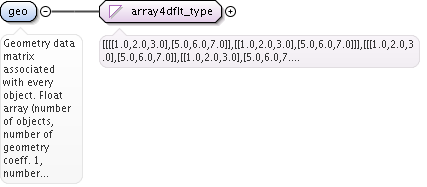
\includegraphics[scale=0.9]{utilities_xsd_Element_geo}
	\caption{CPO $geometry$ data structure}
	\label{fig:cpo_geo1}
\end{figure}

\begin{figure}[ht] \centering
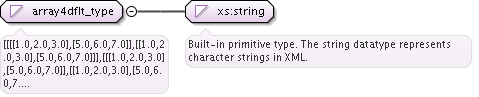
\includegraphics[scale=0.9]{utilities_xsd_Simple_Type_array4dflt_type}
	\caption{CPO $geometry$ array structure}
	\label{fig:cpo_geo2}
\end{figure}

\subsubsection{Geometry and nodes in IDS database}
Similarly to CPO database, the \textbf{geometry} in IDS database is found under subgrid $Nodes$ in $edge\_profiles.ggd(1).grid.space(1).objects\_per\_dimension(c=1).object(k=1).geometry$, where $c$ is \textbf{subgrid class} and $k$ is \textbf{subgrid class object index}, stored as an one-dimensional list as shown in Fig. \ref{fig:IDS_geo1}.

Unlike geometry in CPO database, IDS database has a list of nodes for given subgrid close to geometry dataset, but similarly as in CPO database, we get our geometry using $edge\_profiles...\ .nodes$ data of given subgrid in relation to \\ $edge\_profiles...\ .geometry$ data of the "main" subgrid $Nodes$ so it's not neccessary to define $edge\_profiles...\ .geometry$ for each subgrid and that way we also use less space.



\begin{figure}[ht] \centering
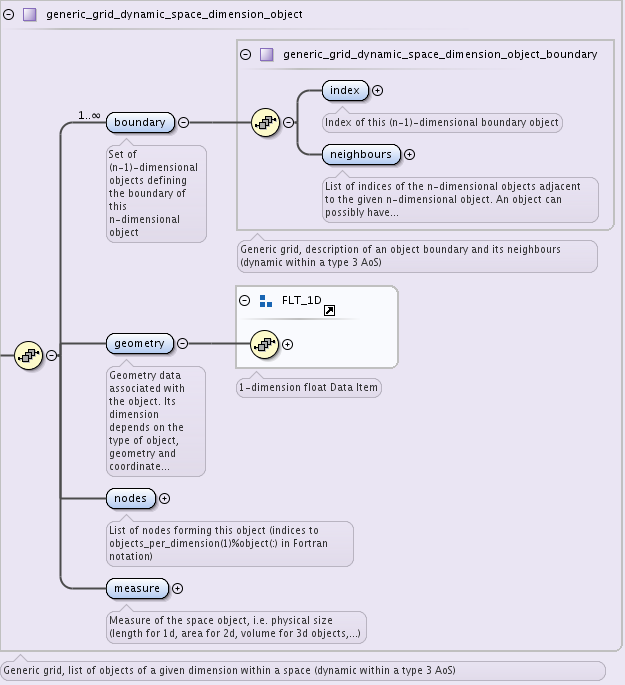
\includegraphics[scale=0.9,trim=3cm 7cm 7cm 9.7cm,clip]{dd_edge_profiles_generic_grid_dynamic_space_dimension_object}
	\caption{IDS $geometry$ data structure}
	\label{fig:IDS_geo1}
\end{figure}

\clearpage

\subsubsection{Important differences between CPO and IDS geometry and nodes data structure}
Because of the 4D array geometry data structure in CPO database, the geometry there can be stored in multi-array structure, while in IDS database it can be stored only as a list of data. To read/write geometry from CPO database we have to state two indices, where first index indicates the node index (goes from $1$ to $n$, where n is number of nodes) while the second index indicates the coordinate (2D: 1 for $x$, 2 for $y$\footnote[1]{0 for $x$ and 1 for $y$ in Python syntax where index counting starts with 0. Also as we're using 2D geometry, the coordinate $z$ is always of value 0 and it's not necessary to specify it.}) in form $\big[[x_1,y_1], [x_2,y_2], ..., [x_n,y_n]\big]$ where $n$ is number of nodes. Because geometry of IDS database is limited to one-dimensional space (list), only one index can be used. The decision was made to write in Fortran notation and in this case read/write to IDS database is done in form $[x_1, x_2, x_3, ..., x_n, y_1, y_2, y_3,... y_n]$ consisting of $2n$ elements, which gives us $n$ nodes. 

We have mentioned, that $geometry$ in CPO databases uses two indices, one of which is node index. IDS database doesn't have this option and it has separate nodes list, located in \\ $edge\_profiles.ggd(1).grid.space(1).objects\_per\_dimension(c)$\\ $.object(k).nodes$ and holds in Fortran notation from 1 to $n$.


\begin{figure}[ht] \centering
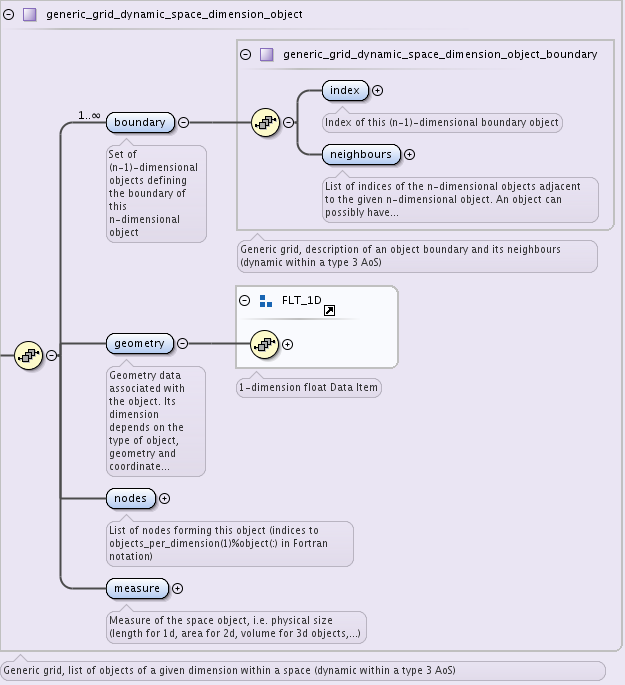
\includegraphics[scale=0.7,trim=3cm 4cm 9cm 17cm,clip]{dd_edge_profiles_generic_grid_dynamic_space_dimension_object}
	\caption{IDS $nodes$ data structure}
	\label{fig:ids_nodes1}
\end{figure}

Also getting the geometry of the $Cells$ subgrid using CPO database was quite problematic to put together. We found only boundary data in \\ $edge.grid.spaces(1).objects(3).boundary$ for which we couldn't find a proper way to use it, instead we managed to correctly construct the $Cells$ subgrid using boundary data from $Edges$ subgrid in \\ $edge.grid.spaces(1).objects(2).boundary$ together with scripting. While converting geometry to IDS, the ordered node indices of $Cells$ subgrid were properly stored under \\ $edge\_profiles.ggd(1).grid.space(1).objects\_per\_dimension(3).object(1).nodes$.

\subsubsection{Converting geometry and nodes from CPO to IDS}

Regarding the previously explained CPO and IDS database structure, transferring geometry data from CPO to IDS database is done by transferring data from:

Geometry and nodes for subgrids class 1 (nodes/points, $c$ = 1):
\begin{itemize}
\item CPO: $edge.grid.spaces(1).objects(2).geo$ to \\
IDS: $edge\_profiles.ggd(1).grid.space(1).objects\_per\_dimension(1).object(1).geometry$
\item CPO: $edge.grid.subgrid(i).list(1).ind$ or $.list(1).indset(1).range$ to \\
IDS: $edge\_profiles.ggd(1).grid.space(1).objects\_per\_dimension(1).object(k).nodes$
\end{itemize}

For subgrids class 2 (edges, $c$ = 2):
\begin{itemize}
\item CPO: $edge.grid.spaces(1).objects(2).boundary$ to \\
IDS: $edge\_profiles.ggd(1).grid.space(1).objects\_per\_dimension(2).object(k).nodes$
\end{itemize}

For subgrids class 3 (cells, $c$ = 3):
\begin{itemize}
\item CPO: Ordered node indices (got with using boundary data from Edges and script) to \\
IDS: $edge_profiles.ggd(1).grid.space(1).objects\_per\_dimension(3).object(1).nodes$
\item CPO: Using ordered node indices and $edge.grid.subgrid(i).list(1).ind$ or $.list(1).indset(1).range$ to \\
IDS: $edge\_profiles.ggd(1).grid.space(1).objects\_per\_dimension(3).object(k).nodes$
\end{itemize}

where $i$ is \textbf{subgrid base index}, $c$ is \textbf{subgrid class index} and $k$ is \textbf{subgrid class object index}.


\clearpage

\addtocontents{toc}{\protect\newpage}

\subsection{\textbf{Electron density and electron temperature }}

\subsubsection{Electron density and electron temperature in CPO database}

In CPO database, electron density and electron temperature datasets are stored under $fluid$ dataset where '$ne$' stands for electron density and '$te$' stands for electron temperature, as shown in Fig. \ref{fig:cpo_fluid}.

\begin{figure}[ht] \centering
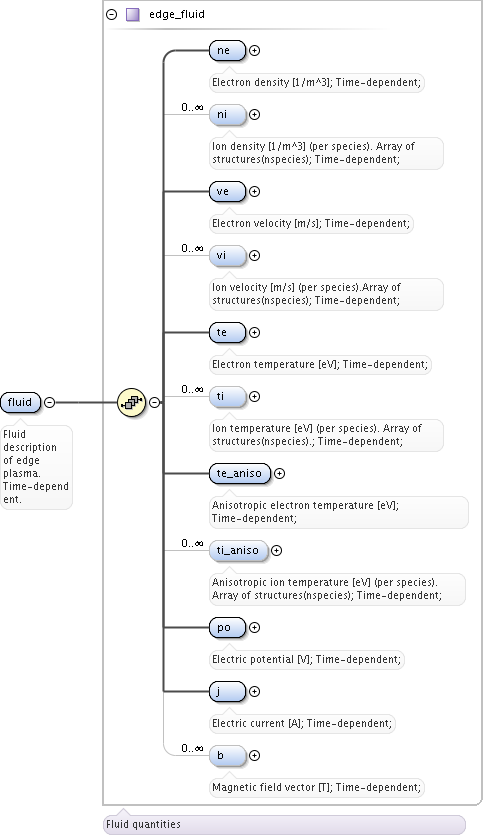
\includegraphics[scale=0.6,trim=0cm 0cm 0cm 0cm,clip]{edge_xsd_Element_fluid}
	\caption{CPO $fluid$ data structure}
	\label{fig:cpo_fluid}
\end{figure}

\clearpage

Furthermore, both electron density and electron temperature dataset structure consists of many subdata sets, $value$ subdata set being one of them \\ (path: $edge.fluid.ne.value(ne\_species\_index)$ where $ne\_species\_index$ goes from 1 to n, where n is number of electron density species), as shown in Fig. \ref{fig:cpo_ne}. In it we can find $subgrid$ data, which is used to store the subgrid base index, and $scalar$ dataset, in which array of data is stored (electron density values in $1/m^3$), as seen on Fig. \ref{fig:cpo_value}.

\begin{figure}[!htb] \centering
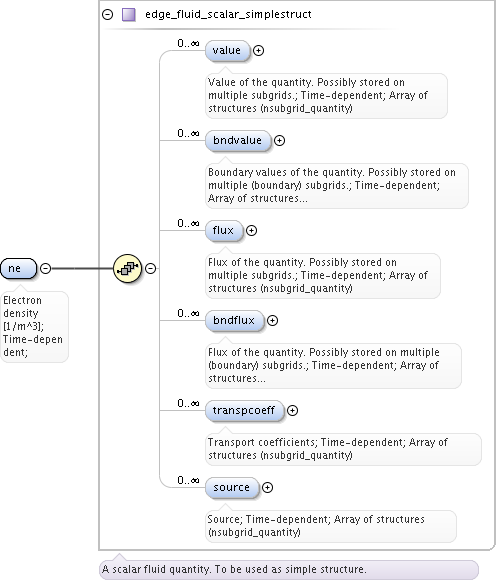
\includegraphics[scale=0.7,trim=0cm 0cm 0cm 0cm,clip]{edge_xsd_Element_ne}
	\caption{CPO $electron density$ data structure}
	\label{fig:cpo_ne}
\end{figure}
\
\begin{figure}[ht] \centering
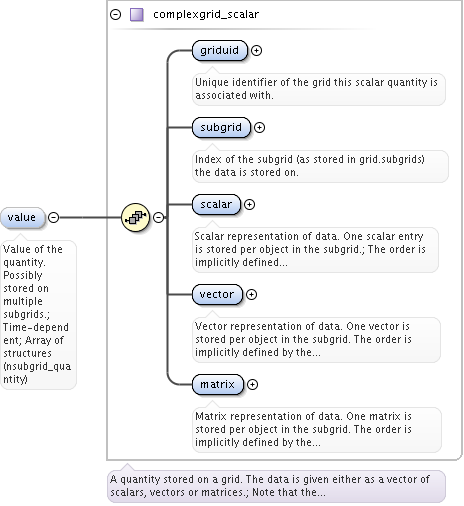
\includegraphics[scale=0.7,trim=0cm 0cm 0cm 0cm,clip]{edge_xsd_Element_value}
	\caption{CPO $value$ data structure}
	\label{fig:cpo_value}
\end{figure}
\
\begin{figure}[ht] \centering
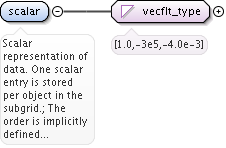
\includegraphics[scale=0.7,trim=0cm 0cm 0cm 0cm,clip]{utilities_xsd_Element_scalar_2}
	\caption{CPO $scalar$ data structure}
	\label{fig:cpo_scalar}
\end{figure}
\
\clearpage
Electron temperature $te$ data set has identical structure as electron density $ne$ data set.

\begin{figure}[ht] \centering
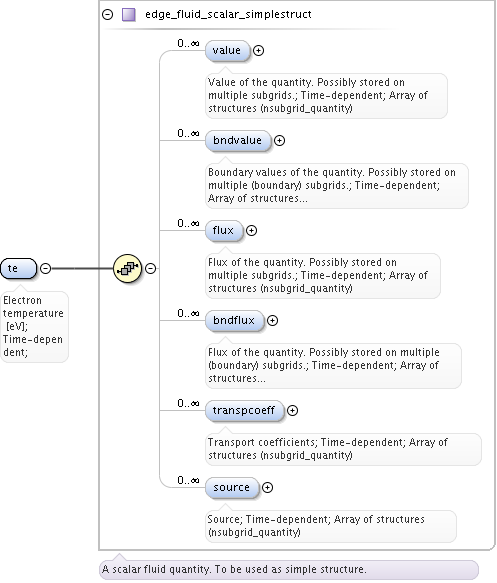
\includegraphics[scale=0.7,trim=0cm 0cm 0cm 0cm,clip]{edge_xsd_Element_te}
	\caption{CPO $electron$ $temperature$ data structure}
	\label{fig:cpo_te}
\end{figure}

\clearpage 

\subsubsection{Electron density and electron temperature in IDS database}

While in CPO database, as already mentioned, electron density $ne$ and electron temperature $te$ datasets are part of $fluid$ dataset, in IDS database are part of $electrons$ dataset 
(path in IDS: $edge\_profiles.ggd(1).electrons$), which furthermore systematically splits to electrons properties datasets, as seen on Fig. \ref{fig:ids_electrons}, with
density (path: $edge\_profiles.ggd(1).electrons.density(ne\_species\_index)$) and temperature (path: $edge\_profiles.ggd(1).electrons.temperature(te\_species\_index)$) included.

\begin{figure}[ht] \centering
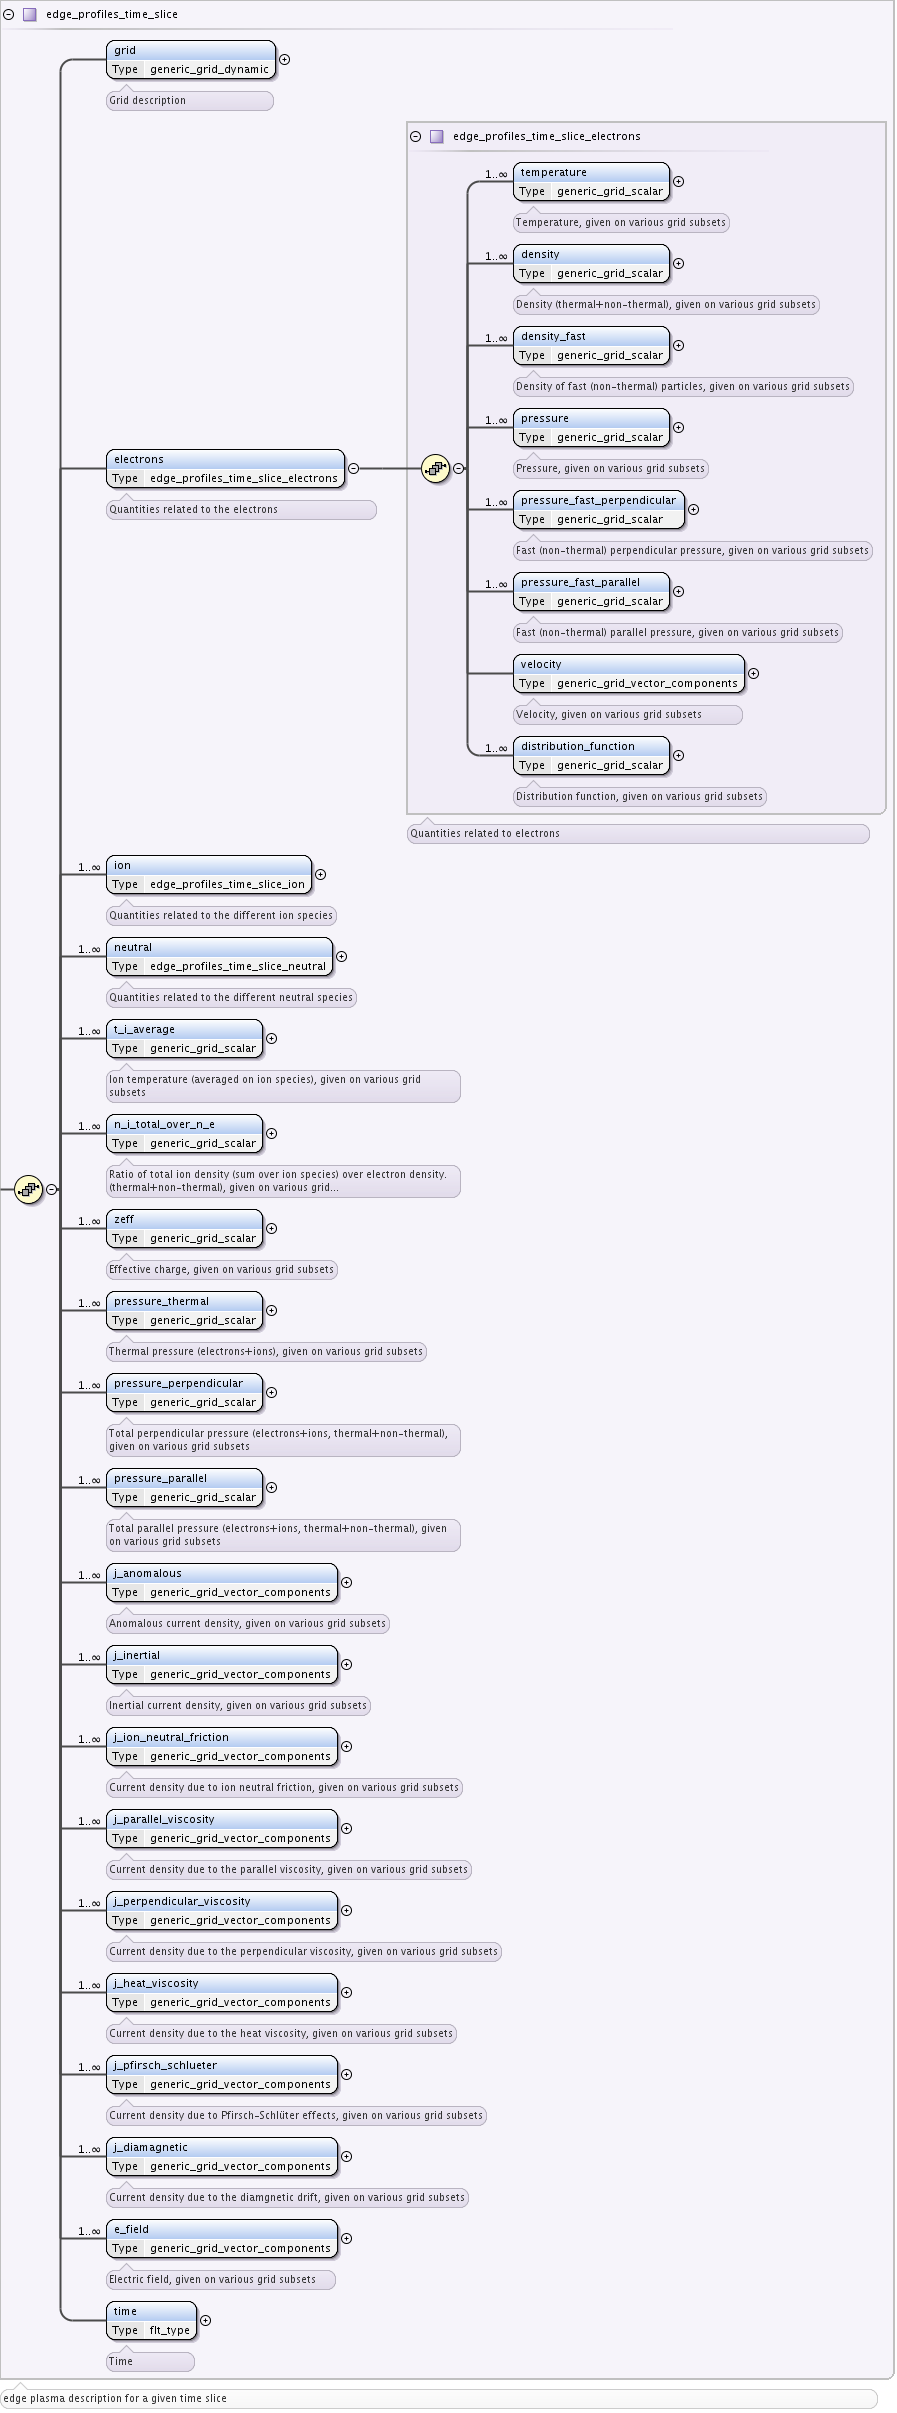
\includegraphics[scale=0.58,trim=3cm 55cm 0cm 4cm,clip]{dd_edge_profiles_edge_profiles_time_slice}
	\caption{IDS $electrons$ data structure}
	\label{fig:ids_electrons}
\end{figure}

\clearpage
The IDS $density$ dataset, shown in Fig. \ref{fig:ids_electron_density} consists of less subdata sets as CPO electron density $ne$ dataset. $Grid\_subset\_index$ (in "Subgrid" and "Geometry and nodes" chapter we called it \textbf{subgrid base index}) and $values$ data in IDS database are taken for being the same datasets as $subgrid$ index and $scalar$ data in CPO database.


\begin{figure}[ht] \centering
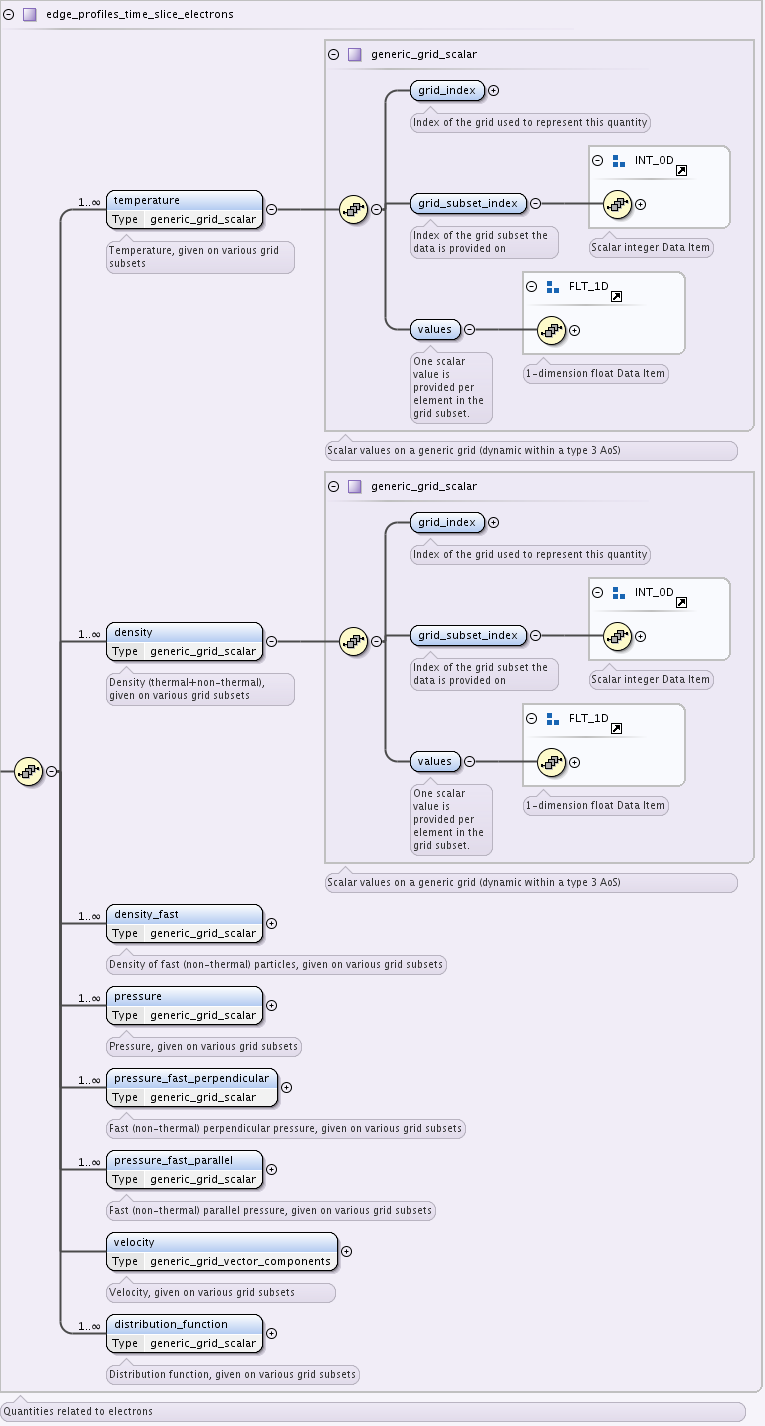
\includegraphics[scale=0.53,trim=2.5cm 18.5cm 0cm 16.5cm,clip]{dd_edge_profiles_edge_profiles_time_slice_electrons}
	\caption{IDS $electron$ $density$ data structure}
	\label{fig:ids_electron_density}
\end{figure}

IDS $temperature$ dataset has the same structure as $density$ dataset as shown in Fig. \ref{fig:ids_electron_temperature}.

\begin{figure}[ht] \centering
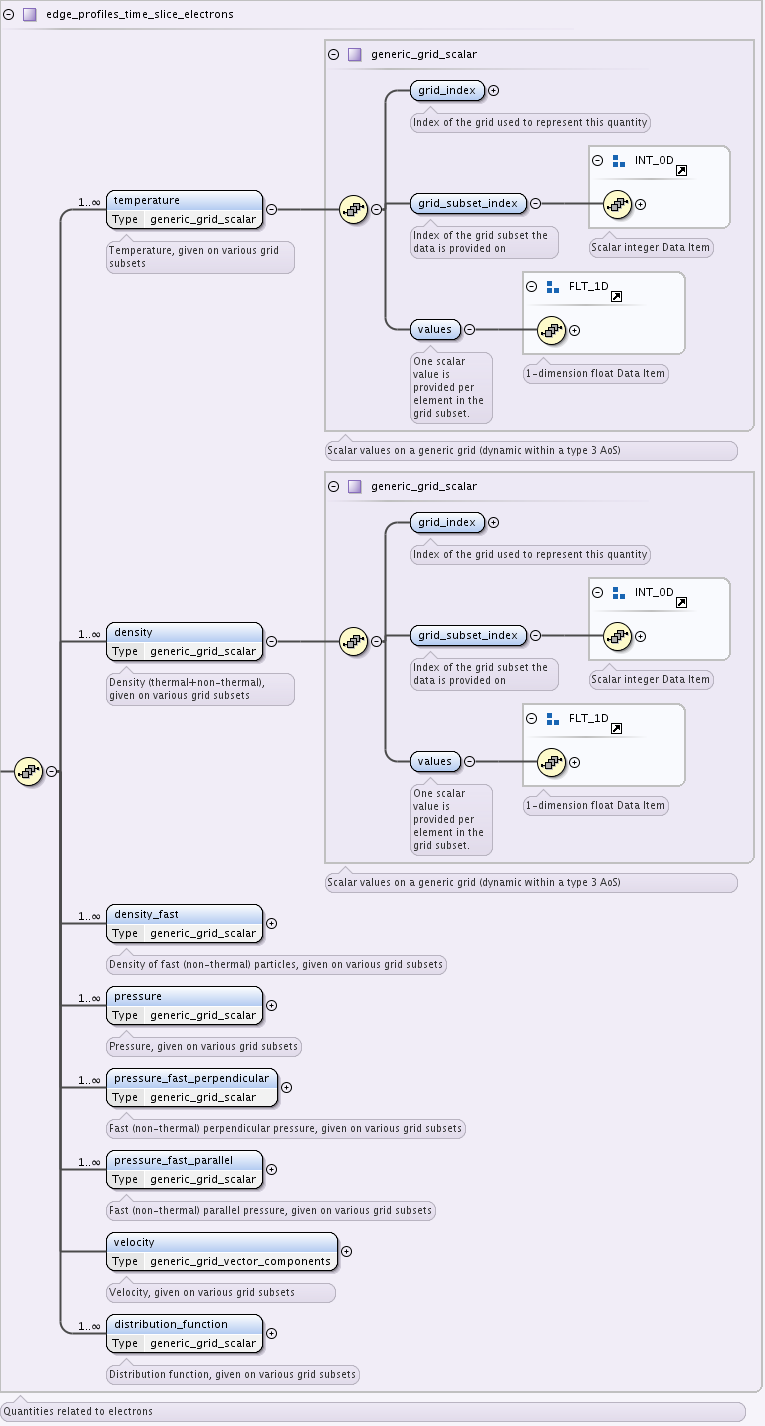
\includegraphics[scale=0.53,trim=2.5cm 33.7cm 0cm 1cm,clip]{dd_edge_profiles_edge_profiles_time_slice_electrons}
	\caption{IDS $electron$ $temperature$ data structure}
	\label{fig:ids_electron_temperature}
\end{figure}

\clearpage 

\subsubsection{Converting electron density and electron temperature scalars from CPO to IDS database}

Regarding the CPO and IDS database structure previously explained, transferring electrons density and temperature data from CPO to IDS database is done by transferring data from

\begin{itemize}
\item CPO: $ edge.fluid.ne.value(m).subgrid$ to \\
IDS: $edge\_profiles.ggd(1).electrons.density(i).grid\_subset\_index $ (electron density subgrid/subset index), \\

\item CPO: $ edge.fluid.ne.value(m).scalar(j)$ to \\
IDS:  $edge\_profiles.ggd(1).electrons.density(m).values(j)$ (electron density values), \\

\item CPO: $edge.fluid.te.value(m).subgrid$  to \\  IDS: $edge\_profiles.ggd(1).electrons.temperature(m).grid\_subset\_index$ (electron temperature subgrid/subset index) and \\

\item CPO: $ edge.fluid.te.value(m).scalar(j)$  to \\
IDS: $edge\_profiles.ggd(1).electrons.temperature(m).values(j)$ (electron temperature values),
\end{itemize}
where $m$ is \textbf{electron density/temperature species index} and $j$ is \textbf{scalar index}.

Moreover, because in IDS we don't have a space to store list of indices for $Core$, $SOL$, $Inner$ $divertor$ and $Outer$ $divertor$ subgrids, corresponding to $Cells$ subgrid (all of them are class 3) as in CPO database (found in $edge.grid.subgrid(i).list(1).ind$ or $.list(1).indset(1).range$), which would be used to properly connect subgrid geometry and subgrid scalars, we decided to create additional 4 electron density and electron temperature species, define proper $grid\_subset\_index$ and, using list of indices from CPO and scalars of $Cells$ subgrid, store the scalars the same way as for previous electron density and electron temperature species.

\clearpage


\subsection{\textbf{Ion density and ion temperature}}

\subsubsection{Ion density and ion temperature in CPO database}

In CPO database, the same as electron density $ne$ and electron temperature $te$, also ion density $ni$ and ion temperature $ti$ are part of $fluid$ database, as already previously shown in Fig. \ref{fig:cpo_fluid}, and have also the same structure, as seen comparing figures Fig. \ref{fig:cpo_ne} and \ref{fig:cpo_te} with  Fig. \ref{fig:cpo_ni} and \ref{fig:cpo_ti}.

\begin{figure}[ht] \centering
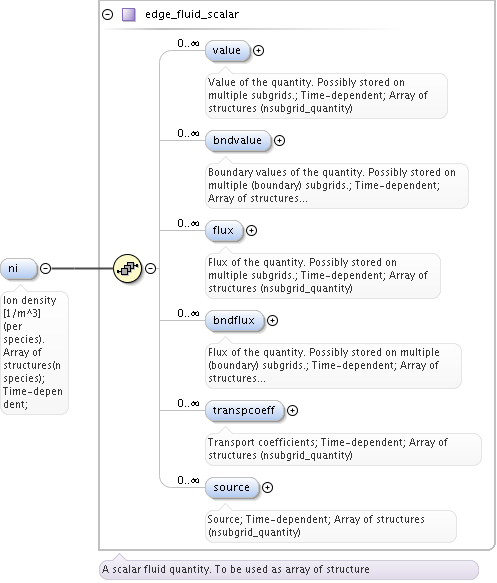
\includegraphics[scale=0.6,trim=0cm 0cm 0cm 0cm,clip]{edge_xsd_Element_ni}
	\caption{CPO $ion$ $density$ data structure}
	\label{fig:cpo_ni}
\end{figure}

\clearpage

But there is one difference. While electrons are only one, we can have many different ions and data corresponding to them, so each ion dataset is set as array of $n$ ion property species. For example, path to ion density data in CPO database would be $edge.fluid.ni(k)$, where $k$ is index corresponding to '$k$' ion.

\begin{figure}[ht] \centering
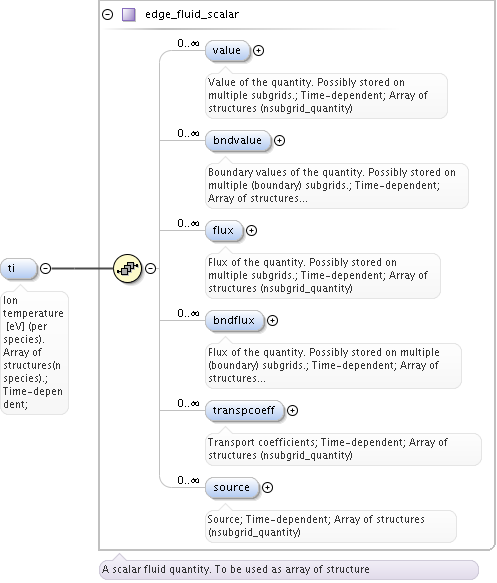
\includegraphics[scale=0.6,trim=0cm 0cm 0cm 0cm,clip]{edge_xsd_Element_ti}
	\caption{CPO $ion$ $temperature$ data structure}
	\label{fig:cpo_ti}
\end{figure}

\subsubsection{Ion density and ion temperature in IDS database}

In IDS database, the structure of ion dataset, shown in Fig. \ref{fig:ids_ions}, is more extensive in comparison with the electrons dataset, shown in Fig. \ref{fig:ids_electrons}, while ion density and ion temperature dataset structure, shown in Fig. \ref{fig:ids_ion_density} and \ref{fig:ids_ion_temperature}, remains the same as structure of electron density and electron temperature dataset, previously shown in Fig. \ref{fig:ids_electron_density} and \ref{fig:ids_electron_temperature}. Also, similarly as in CPO database, $ion$ database is array of $n$ property species.

\begin{figure}[ht] \centering
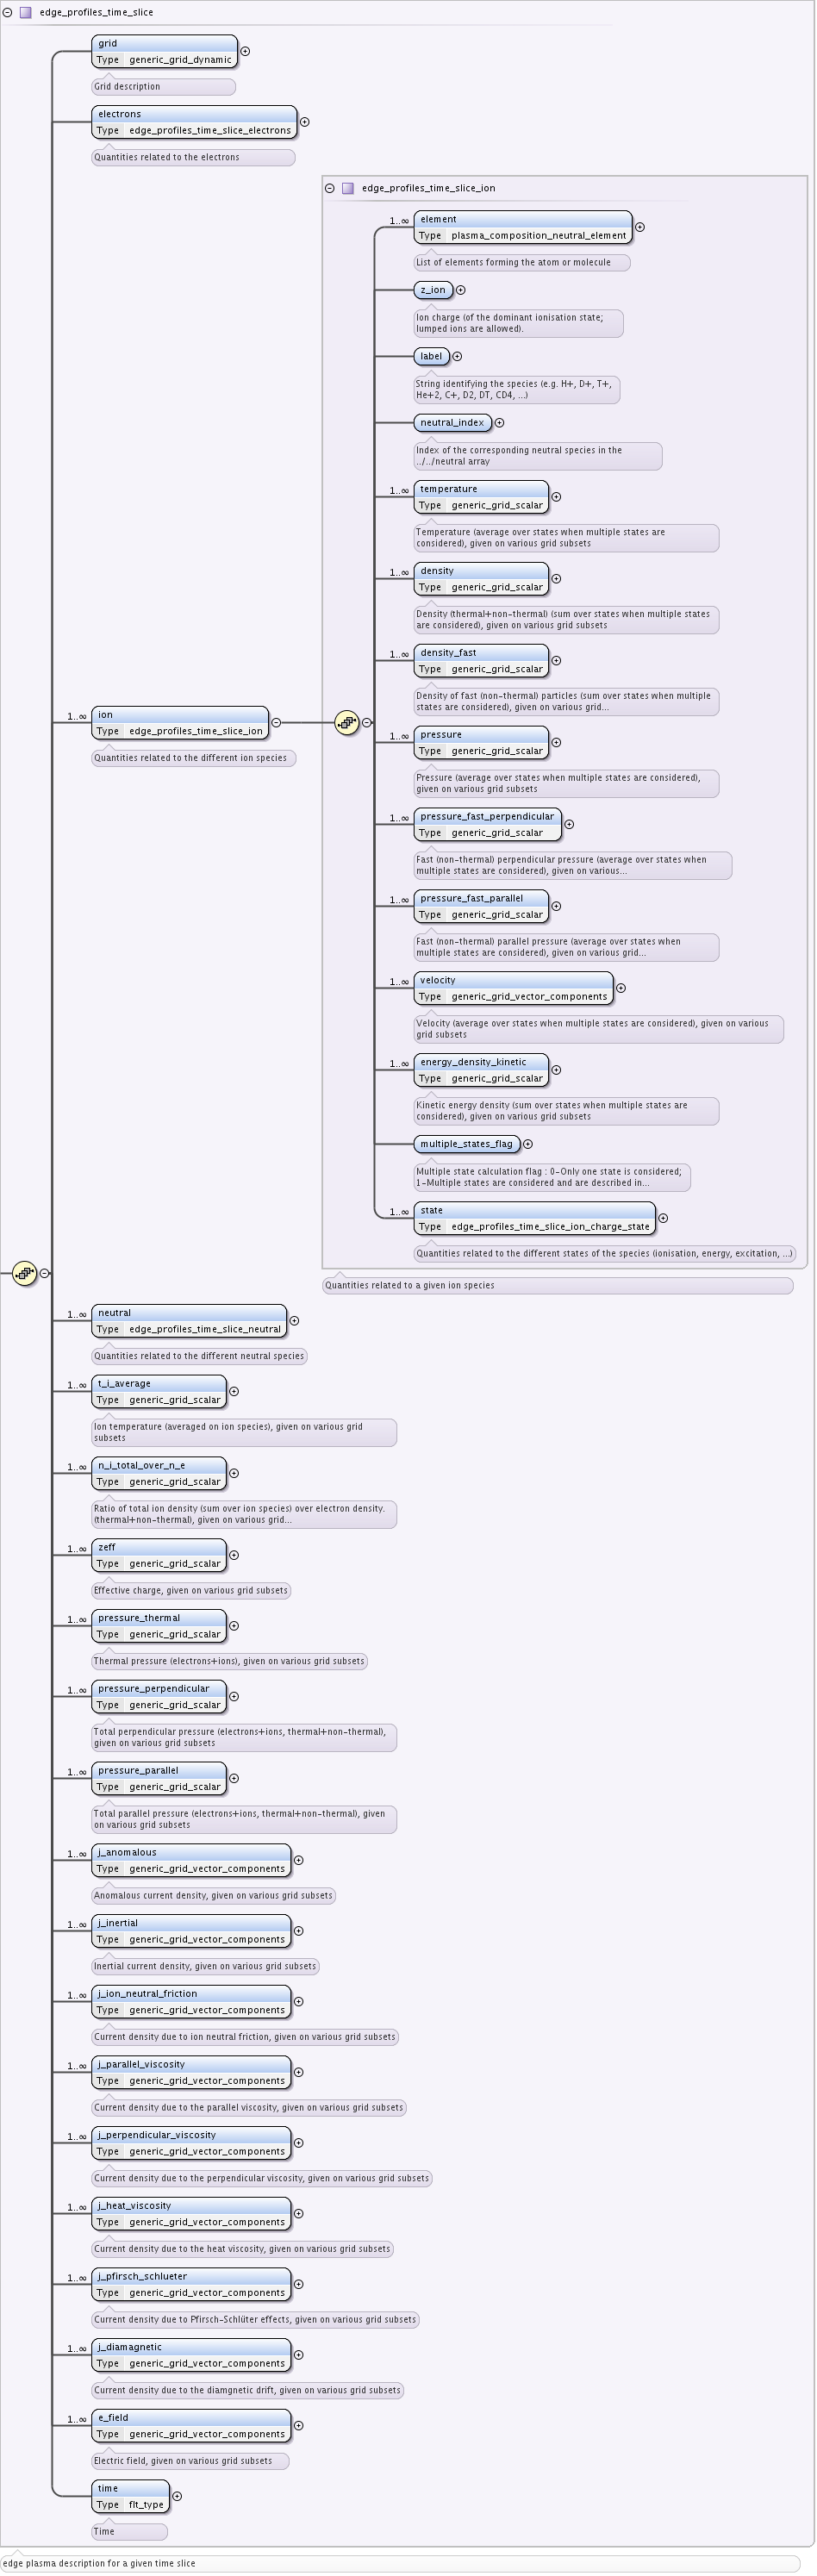
\includegraphics[scale=0.5,trim=2.5cm 52.25cm 0cm 7cm,clip]{dd_edge_profiles_edge_profiles_time_slice2}
	\caption{IDS $ion$ structure}
	\label{fig:ids_ions}
\end{figure}
\clearpage

\begin{figure}[!htb] \centering
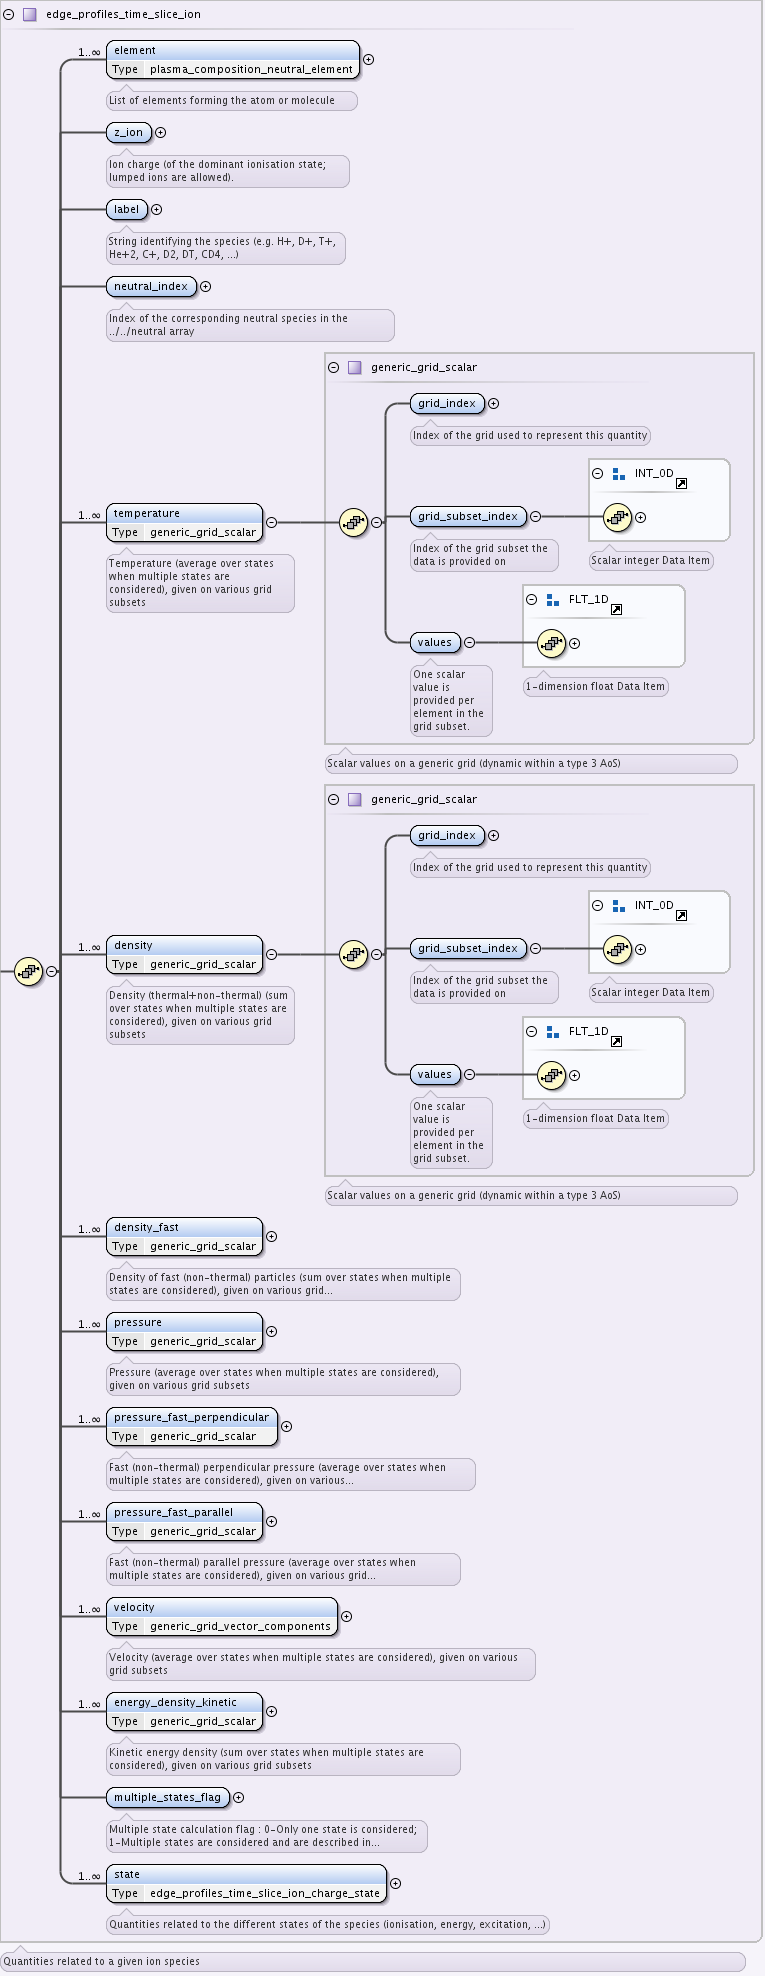
\includegraphics[scale=0.6,trim=2.5cm 28cm 0cm 27.5cm,clip]{dd_edge_profiles_edge_profiles_time_slice_ion}
	\caption{IDS $ion$ $density$ structure}
	\label{fig:ids_ion_density}
\end{figure}

\begin{figure}[!htb] \centering
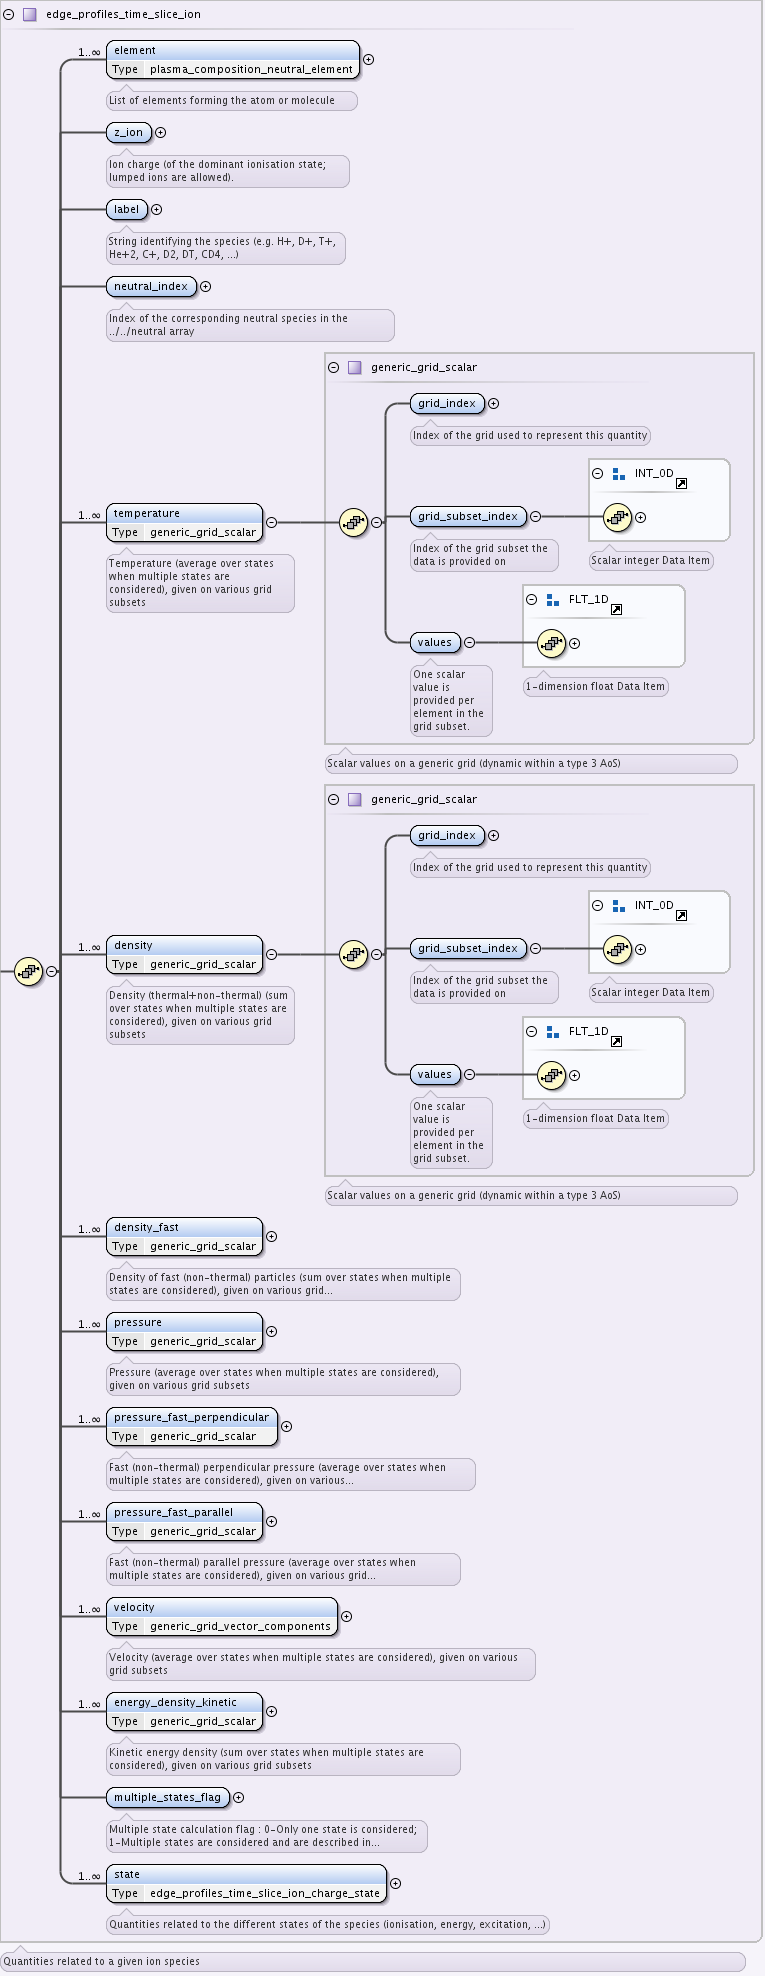
\includegraphics[scale=0.6,trim=2.5cm 43.3cm 0cm 12.3cm,clip]{dd_edge_profiles_edge_profiles_time_slice_ion}
	\caption{IDS $ion$ $temperature$ structure}
	\label{fig:ids_ion_temperature}
\end{figure}

\clearpage

\subsubsection{Converting ion density and ion temperature from CPO to IDS database}

Regarding the CPO and IDS database structure previously explained, transferring ion density and temperature data from CPO to IDS database is done by transferring data from

\begin{itemize}
\item CPO: $ edge.fluid.ni(p).value(m).subgrid$  to \\
IDS: $edge\_profiles.ggd(1).ion(p).density(m).grid\_subset\_index $ (ion density subgrid/subset index), \\

\item CPO: $ edge.fluid.ni(p).value(m).scalar(j)$  to \\
 IDS: $edge\_profiles.ggd(1).ion(k).density(m).values(j)$ (ion density values), \\

\item CPO: $ edge.fluid.ti(p).value(i).subgrid$ to \\  IDS: $edge\_profiles.ggd(1).ion(p).temperature(m).grid\_subset\_index$ (ion temperature subgrid/subset index) and \\

\item CPO: $ edge.fluid.ti(p).value(m).scalar(j)$  to \\
IDS: $edge\_profiles.ggd(1).ion(p).temperature(m).values(j)$ (ion temperature values),
\end{itemize}
where $p$ is \textbf{ion index}, $m$ is \textbf{ion density/temperature species index} and $j$ is \textbf{scalar index}.

Moreover, the same as discussed in previous section about converting electron \\ density/temperature scalars, in IDS database we don't have place to store the list of indices for $Core$, $SOL$, $Inner$ $divertor$ and $Outer$ $divertor$ subgrids, corresponding to $Cells$ subgrid (class 3 subgrids) as in CPO database. The issue was solved in the same way as for electron properties. For each ion dataset we created additional 4 ion density and ion temperature species, defined proper $grid\_subset\_index$ and, using list of indices from CPO and scalars of $Cells$ subgrid, store the scalars the same way as for previous ion density and ion temperature species.

\end{document}
